\documentclass{sig-alternate-2015}

%\clubpenalty=10000 
%\widowpenalty = 10000


\usepackage{graphicx}
\usepackage{caption}
\usepackage{subcaption}
\usepackage{balance}
\usepackage{algpseudocode}
\usepackage{algorithm}
\usepackage{enumitem}
\usepackage{multirow}


\usepackage{color}
\usepackage{tabularx}
\usepackage[table]{xcolor}

\usepackage{framed}

\newtheorem{definition}{Definition}
\newtheorem{problem}{Problem}
\newtheorem{lemma}{Lemma}

\newcommand{\mf}{\ensuremath{\mathfrak}}
\newcommand{\rv}{\ensuremath{\mathcal}}
\newcommand{\rb}{\ensuremath{\mathbf}}
\newcommand{\norm}[1]{\left\lVert #1 \right\rVert}
\newcommand{\nott}{\ensuremath{\overline{t}}}

\newenvironment{itemize0}
{ 
    \begin{itemize}
        \setlength{\topsep}{0pt}
        \setlength{\itemsep}{0pt}
        \setlength{\parskip}{0pt}
        \setlength{\parsep}{0pt} 
}
{ \end{itemize}  }


\begin{document}

\title{``Hey Ziggy, What Am I Looking At?''\\
Describing Tuples for Data Explorers}

\numberofauthors{3}
\author{
\alignauthor
Thibault Sellam\\
       \affaddr{CWI\\Amsterdam, the Netherlands}\\
       \email{thibault.sellam@cwi.nl}
\alignauthor
Emmanuel M\"uller\\
    \affaddr{HPI\\Potsdam, Germany}\\
     \email{emmanuel.mueller@kit.edu}
\alignauthor
Martin Kersten\\
       \affaddr{CWI\\Amsterdam, the Netherlands}\\
       \email{martin.kersten@cwi.nl}
}

\maketitle

\begin{abstract} 
The aim of data exploration is to get acquainted with an unfamiliar database.
Typically, explorers operate by trial and error: they submit a query, study the
result, and refine their query subsequently. In this paper, we investigate how
to help them understand their query results. In particular, we focus on medium
to high dimension spaces: if the database contains dozens or hundreds of
columns, which variables should they inspect? We propose to detect subspaces
in which the users' selection has an unusual distribution compared to the rest
of the database. From this idea, we built Ziggy, a tuple description engine.
Ziggy can detect informative subspaces, and it can explain why it recommends
them with natural language and visualizations. Thus it engages users in a
veritable conversation with their data exploration tool.  We first present the
general problem of characteri\-zing tuples with multiple views. We then describe
Ziggy in detail. Finally, we showcase our system with a real-life use case, and
evaluate it with a wide range of real and synthetic data.
\end{abstract}


\category{H.2.8}{Database Applications}{Data mining}
\keywords{Data exploration, subspace search, data description}

\section{Introduction}
\label{sec:introdction}
Data exploration has gained lots of attentions over the last few years. The
main challenge is to support users with little prior knowledge, and no clear
objective. Such users may need a preliminary impression of the data before
engaging into more structured tasks, or they may  seek inspiration for original
hypotheses. Consequently, several authors have proposed systems to
``play'' with the data~\cite{abouzied2012dataplay, sellam2013meet,
liarou2014dbtouch, dimitriadou2014explore}. Typically, these systems propose
some graphical interface through which users can create, visualize and modify
selections of tuples quickly. Thus, explorers are engaged in a tight
trial-and-error loop, through which they discover their datasets. 

These approaches rely on a crucial assumption: they suppose that if a user sees
an interesting set of tuples (e.g., through tables or visualizations), they
will recognize it immediately, and think ``aha, this is interesting''. This
assumption may hold with small datasets, but it breaks down in higher
dimensions. What if the dataset contains several dozens, or hundreds of
columns? Which dimensions are informative? Furthermore, which
\emph{combinations} of columns are informative? In a data exploration setting,
we cannot assume that the users know which variables to look at. Yet, studying
each possibility in turn can turn out to be a slow, tedious
process. This beats the purpose of a data exploration system.
\begin{framed}
    \everypar={{\setbox0=\lastbox}\everypar{}}
    In a data exploration context, how can we describe a set of tuples with
    more than a dozen columns?
\end{framed}

The straightforward approach is to use multidimensional visualizations such as
parallel coordinates or small multiples. Unfortunately, these methods tend to
show every possible aspect of the data, thus they do not scale well. For
instance, we would need at least 50 small multiples to visualize a dataset with
only 10 columns. Dimensionality reduction algorithms such as PCA or ICA are
also common, but they are oblivious to the user's selection, hence they may
miss interesting aspects.  Besides, their output are harder to interpret.

In this paper we introduce our approach, \emph{multi-view subset
characterization}. The key idea is to detect subspaces inside which the user's
selection has an unusual distribution compared to the rest of the database.  To
illustrate our point, we present Ziggy, a \emph{subset description engine}.
\emph{For a given subset of a database, Ziggy can automatically generate a
description of the tuples with natural language and visualizations.} Thus,
plugged on top of a database engine, Ziggy can veritably simulate a
conversation with the user: the user issues queries, and Ziggy replies in
natural language. Our system can process more than a hundred columns in a few
seconds, and it can cope with both numerical and nominal data. Here is an
example of Ziggy's descriptions:
\begin{quote}
    Take a look at columns X, Y and Z. On X, and Y, your selection has a very
    low value. On column Z, your selection has a fairly low value, with high
    concentration. The correlation between Y and Z is unusually strong.\\
    You can also take a look at columns T. On this column, the
    values ``xxx'', ``yyy'', and ``ttt'' are underrepresented, while the values
    ``aa'' and ``bb'' are overrepresented.
\end{quote}

%Several authors have tackled similar problems in the
%past~\cite{angiulli2009detecting, knorr1999finding, loekito2008mining,
%webb2008detecting}. None of them use natural language.
%
Our paper is built as follows. First, we discuss how to detect database views
in which a given set of tuple is ``special''. We expose the problem in its
generality, and discuss its relation to other methods, such as feature
selection. Second, we instantiate our problem with a custom objective function,
designed to yield interpretable results. Our function aggregates several
well-known statistical tests, carried out in a systematic, purposely
brute-force way.  Finally, we discuss how to describe the views with natural
language, and how to check the robustness of our results.

\section{General Problem Formulation}
\label{sec:problem}
\begin{figure}
  \centering
  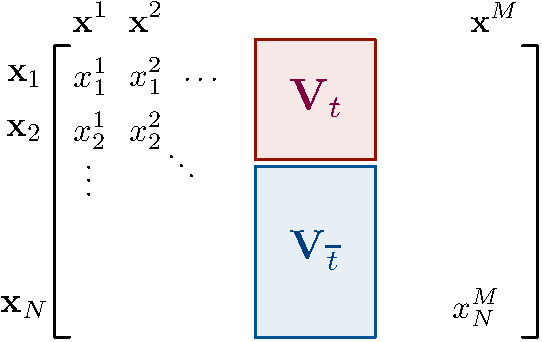
\includegraphics[width=0.6\columnwidth]{Figures/Notations}
  \caption{Notations.}
  \label{pic:notations}
\end{figure}

{\color{red} Here, I need to give a high level introduction to motivate our
approach - in particular why we use multiple views}

Let the matrix $\rb{D}$ with $M$ columns and $N$ rows represent our database.
We suppose that each tuple $\rb{x}_n = (x^1_n, \dots, x^M_n)^\top$ in the
database is an iid. sample from some unknown distribution
$p(\rb{x}_n)=p(\rb{x})$. We represent each column with a vector $\rb{x}^{m}=
(x^m_1, \dots, x^m_N)^\top$.  The user specifies a ``special'' selection of
tuples, described by the vector $\rb{t} = (t_1, \ldots, t_n)^\top$: $t_i=1$ if
the tuple is chosen, 0 otherwise. We refer to the tuples in the selection as
${\rb{D}}_t$, and the remaining tuples as ${\rb{D}}_{\overline{t}}$. We refer
to the underlying distributions as $p(\rb{x}|t)$ and $p(\rb{x}|\overline{t})$
respectively. We illustrate these notations with Figure~\ref{pic:notations}.

Our model is based on a user-specified \textbf{mass dissimilarity measure}
$\mf{D}(\rb{D}, \rb{D}')$, which measures the difference between two groups of
tuples. If the rows of $\rb{D}$ and $\rb{D}'$ are sampled from the same
distribution, then $\mf{D}$ is very close to 0. If
not, $\mf{D}$ grows with the dissimilarity of the distributions.
Figure~\ref{pic:sameMean} gives an example of the latter case.  Here are some
possible choices:
\begin{itemize}
    \item A simple option is to use the distance between centroids (possibly
        weighted by the observed covariance)
    \item A more general option is to estimate the Kullback-Leibler divergence:
        $\mf{D}(\rb{D}, \rb{D}') \equiv KL(\hat{p}(\rb{x});
        \hat{p}'(\rb{x}'))$, where $\hat{p}(\rb{x})$ and $\hat{p}'(\rb{x}')$
        are density estimators. This approach is more general, as it can cope
        with both continuous and categorical variables.
    \item In the next section, we introduce our own mass dissimilarity.
\end{itemize}
Knowing this function $\mf{D}$, we can already propose a first, naive,
formulation of our problem. \emph{We want to find groups of variables on which the
distribution of the chosen tuples is different from that of the rest of the
data}.
\begin{problem}
    Consider a distribution dissimilarity function $\mf{D}$ and two integers
    $K$ and $D$. Find the top $K$ distinct views $\rb{D}^i = [\rb{x}^1, \dots,
    \rb{x}^d]$ with at most $D$ dimensions which maximize: $ \mf{D}\big(
    \rb{D}^i_t ; \rb{D}^i_{\overline{t}} \big)$ (ignoring column permutations).
\end{problem}
\begin{figure}
  \centering
  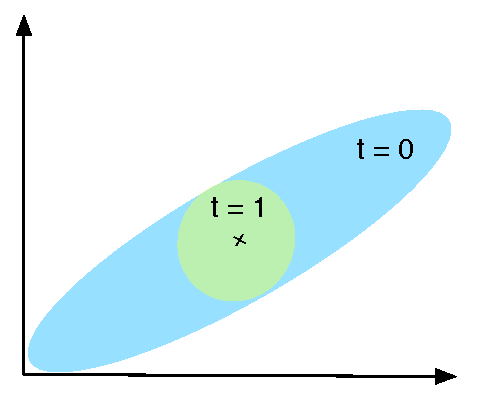
\includegraphics[width=0.5\columnwidth]{Figures/SameMean}
  \caption{Example of interesting view. {\color{red}This figure is really ugly.}}
  \label{pic:sameMean}
\end{figure}

This approach is simple, but it can lead to redundancy: a small number
of good columns may dominate the results and appear in all $K$ views. In a data
exploration scenario, users may value \emph{diversity}, even if the views are
sub-optimal. To enforce this requirement, we introduce a penalty factor in our
objective function. 

To measure redundancy, we propose to use statistical dependency. The rationale
is the following: if two sets of columns are tightly correlated, then there is
a high chance that they describe the same property of the ``real world''.
Oppositely, if they are independent, then they probably convey different types
of information. From this observation, we introduce a new version of our
problem: we seek views which maximize the distance statistic, while minimizing
inter-view dependency.  We define this problem in a recursive way:
\begin{problem}
    Suppose that we have already detected $i-1$ views, $i > 1$. We obtain
    $\rb{D}^{1..i-1} =
    [\rb{D}^1, \ldots, \rb{D}^{i-1}]$ by concatenating these views. Let
    $\mf{S}$ describe a statistical dependency measure. Given a
    positive real $\lambda$, find the view $\rb{D}^{i}$ with at most $D$
    columns which maximizes:
        \begin{equation}
            \label{prob1}
            \mf{D}\big( \rb{D}^{i}_t  ; \rb{D}^{i}_{\overline{t}} \big) - 
            \lambda \cdot \mf{S} ( \rb{D}^{i} ; \rb{D}^{1..i-1})
        \end{equation}
\end{problem}
The statistics literature presents many options to instantiate the dependency
measure $\mf{S}$. Well established examples are the correlation coefficient, or
the mutual information. We will present our own function in
Section~\ref{sec:dependency}.

In Equation~\ref{prob1}, the parameter $\lambda$ controls the trade-off between
mass distance and view diversity: a high value enforces that that the view are
diverse, while a low value expresses our preference for maximizing $\mf{D}(
\rb{D}^{i}_t  ; \rb{D}^{i}_{\overline{t}})$. In practice, this parameter is
not convenient because it has no intuitive scale. For some $L$, an
equivalent way to express our problem is the following:
\begin{equation}
    \label{prob2}
    \begin{aligned}
        & \text{Argmax}_{\rb{D}^{i}} 
            & \mf{D}\big( \rb{D}^{i}_t  ; \rb{D}^{i}_{\overline{t}} \big)\\
        & \text{s.t.} 
        &\mf{S} ( \rb{D}^{i} ; \rb{D}^{1..i-1}) & < L\\ 
    \end{aligned}
\end{equation}
Equation~\ref{prob1} in the Lagrangian of Equation~\ref{prob2}, up to a
negligible additive constant. We prefer this form because the trade-off
parameter $L$ has the same scale as $\mf{S} ( \rb{D}^{i} ; \rb{D}^{1..i-1}) $.
For example, if we instantiate $\mf{S}$ with the linear correlation, then $L$
will simply describe the maximal acceptable correlation between $\rb{D}^{i}$
and $\rb{D}^{1..i-1}$.

At this point, we notice that our problem is very to close to \emph{feature
selection}. Feature selection seeks columns of $\rb{D}$ from which we can
predict $\rb{t}$. Ultimately, the goal is to estimate $p(t|\rb{x})$. Our
problem is symmetric: we seek columns of $\rb{D}$ which are influenced by
$\rb{t}$. Hence, we focus on $p(\rb{x}|t)$. According to Bayes' theorem, these
two problems are equivalent. And indeed, some feature selection methods, such
as LDA, are also based on $p(\rb{x}|t)$. But the differences do not stop here.
Recall we focus on interpretation, while feature selection algorithms
target prediction. Therefore, we seek a few, non-redundant views, while
classic algorithms focus on single, potentially complex views. Also, most
feature selection algorithms optimize class separability. In this paper, we are
interested in any kind of dissimilarity. For instance, most feature selection
algorithms would reject the view presented in Figure~\ref{pic:sameMean}. For
us, this view is perfectly acceptable. 
\begin{table*}[t]
    \centering
    \begin{tabular}{|c|c|c|c|p{7cm}|}
      \hline
      Property & Type 1 & Type 2 & Zig-Component & Comments\\
      \hline
      Mean        & Contin.  & - &
      $  \mf{z}_\mu (d_t, d_{\nott}) = \frac{\mu_t - \mu_{\overline{t}}}{
      \sigma_{\overline{t}}}$&  Known as Glass' $\Delta$  \\

     Stand. Dev.& Contin.  & - &
      $ \mf{z}_\sigma (d_t, d_{\nott}) =  \frac{\sigma_T - \sigma_{\overline{t}}}{ \sigma_{\overline{t}}}$ & \\
    
      Frequencies & Discrete & - & 
    $  \mf{z}_\chi (d_t, d_{\nott}) =  \sqrt{\frac{\chi^2}{N(k - 1)}}$ & Known
          as Cram\'er's V, $\chi^2$ represents the value of the
          goodness-of-fit $\chi^2$ statistic between $d_t$ and $d_{\nott}$, $k$
          is the number of distinct values.\\
      
          \hline
      Dependence  & Contin. & Contin & $
      \mf{z}_r ([d_t, d'_t ], [d_{\nott}, d'_{\nott} ]) =     r_t - r_{\overline{t}} $ & 
      $r_t$ (resp. $r_{\nott}$) is the correlation coefficient between $d_t$
      and  $d'_t$ (resp   $d_{\nott}$ and  $d'_{\nott}$ ) \\
      Dependence  & Discrete & Both &

      $ \mf{z}_V ([d_t, d'_t ], [d_{\nott}, d'_{\nott} ]) = V_t - V_{\overline{t}} $ &
           $V_T$ (resp. $V_{\nott}$) is Cramer's V coefficient between $d_t$
      and  $d'_t$ (resp   $d_{\nott}$ and  $d'_{\nott}$ ) \\ 
      \hline
    \end{tabular}
\caption{Our choice of Zig-Components for different data types. The variable
    $d$ and $d'$ represent columns with mean $\mu$ and
    standard deviation $\sigma$. Note that in the bivariate case we actually compute statistics of statistics.}
    \label{tab:dissim}
\end{table*}

\section{Instantiation: Meet Ziggy}
\label{sec:instantiation}
\subsection{Explainable Mass Dissimilarity}
\label{sec:explain}
We now discuss how to instantiate the function~$\mf{D}$. In principle, we could
borrow a very general divergence measure from the statistics literature, such
as the KL-divergence. However, these measurements operate as ``black boxes'':
they describe the intensity of the differences, but they do not explain how the
tuples differ. Our approach is different: we introduce the
\textbf{Zig-Dissimilarity} (Ziggy's Dissimilarity), a purposely naive, but
completely \emph{explainable}  mass dissimilarity measure.

The main idea behind the Zig-Dissimilarity is to compute several simple,
interpretable indicators of difference, called \textbf{Zig-Components}, and
aggregate them with a weighted sum.  Consider for instance two sets of tuples
$\rb{D}_t$ and $\rb{D}_{\nott}$ with $M_\rb{D}$ columns. If these sets have the
same average for every column, then they probably come from the same
distribution. Oppositely, if the averages are different, then they may come
from different distributions. From this observation, we build a simple
dissimilarity measure: for each column $m$, we compute the differences between
the means $\mu^m_t - \mu^m_{\nott}$. We obtain a vector of $M_D$ 
Zig-Components. We could add more components by testing other properties: for example, we
could measure the difference between the variance of each columns.
We then aggregate these components into one composite
indicator: this is is the Zig-Dissimilarity.

\begin{definition}
    A Zig-Component is a function $\mf{z} : \rb{D}\times\rb{D} \to \mathbb{R}$
    which describes one difference between two sets of tuples. If the tuples
    are similar, then $\mf{z}(\rb{D}_t, \rb{D}_{\nott}) = 0$. If not,
    the magnitude of $\mf{z}(\rb{D}_t, \rb{D}_{\nott})$ varies with the strength
    of the difference.
\end{definition}
For the sake of presentation, we will abbreviate $\mf{z}(\rb{D}_t,
\rb{D}_{\nott})$ as~$\mf{z}$.

In our implementation, we combined five types of Zig-Com\-po\-nents, summarized in
Table~\ref{tab:dissim}.  Most of them come from statistics textbooks,
where they are referred to as \emph{effect sizes}. We chose these
indicators because they have intuitive interpretations, as well as
known asymptotic properties (we will use these properties in
Section~\ref{sec:validation}). Observe how Ziggy deals with categorical data:
for each subset $\rb{D}_t$ and $\rb{D}_{\nott}$, it computes one histogram per column, and estimates the
difference in distribution with a normalized variant of the $\chi^2$ 
statistic. Ziggy also computes bivariate components: in this case it
compares columns by groups of two. The idea is to check which correlations are
present in one set and not in the other, or alternatively  which correlations
are strengthened across the datasets. Finally, note that most effects are
normalized to vary between -1 and 1, but not all of them (for instance, the
difference of standard deviations can in theory be infinitely large). None of these
functions are symmetric, and most of them change sign according to the
direction of the underlying effect.

Once we computed the Zig-Components $\mf{z}_1, \ldots, \mf{z}_Z$, we obtain the
Zig-Dissimilarity as follows. First, we compute the absolute values
$|\mf{z}_1|, \ldots, |\mf{z}_Z|$ for each component. We then normalize the
values across components of same type. We obtain a set of intermediary scores
$z_1, \ldots, z_Z$. Finally we aggregate these scores with a weighted sum.
These operations give us a scalar indicator, which summarizes several specific
differences between the two sets of tuples.

\begin{definition}
    Let $z_1, \ldots, z_Z$ represent a set of normalized absolute values of
    zig-components, and $w_1, \ldots, w_Z$ a set of user-defined weights.  We
    define the Zig-Dissimilarity as follows: 
    \begin{equation}
    \mf{Z}(z_1, \ldots, z_Z) \equiv \sum_{k \in [1, Z]} w_k \cdot z_k
    \end{equation}
\end{definition}
We insist that the Zig-Components must be normalized before the aggregation.
In the general case, we cannot assume that the scores are commensurate. And
even if they are, it is not always clear whether aggregating them makes sense.
For instance, in Table~\ref{tab:dissim}, all the scores involving numerical
variables are expressed as multiples of $\sigma_{\nott}$. Yet, they all
describe a different property. Admittedly, we could not establish whether summing
them directly would produce meaningful results.

The aim of the weights $w_k$ is to balance the effects across column types. For
instance, we measure two components for the numerical columns, and only one for
categorical data.  Thus, we set $w_k = 1/2$ for the former case and $w_k = 1$
for the latter.  These parameters also let users express their preferences: for
example, a novice user may value one-dimension Zig-Components over those based
on correlation.

Table~\ref{tab:dissim} shows that we measure differences in spaces of one and
two dimensions only.  In principle, we could test spaces with more dimensions.
We chose not to do so, for two practical reasons. First, we suppose that
relationships in three dimensions or more are harder to convey and understand
in natural language.  Second, the number of relationships to be tested grows
exponentially with the dimensionality of the test. This harms Ziggy's runtime,
and it leads to much longer outputs. Nevertheless, this means in no way that
Ziggy's views are limited to two dimensions. In fact, our experiments will
reveal that this Naive Bayes-like assumption has little practical effect on the
accuracy of our model.


\subsection{Dependency Measure}
\label{sec:dependency}

Our aim is to find sets of columns which maximize the dissimilarity $\mf{D}$
between the selected tuples, and minimize the redundancy $\mf{S}$ with the
previously detected views. We introduced a measure of dissimilarity in the
previous sections. We now present two instantiations for the measure of
redundancy, $\mf{S}_{hard}$ and $\mf{S}_{soft}$. 
These functions vary between 0 and 1, 0 indicating no
correlation and 1 indicating maximal correlation. Both measures are a variant
of the same principle, and we will refer to them collectively as $\mf{S}_{Zig}$.

Let $\rb{D}$ and $\rb{D}'$ represent two views. The measure $\mf{S}_{hard}$
describes the worse case scenario: we compute the dependency between every
column of $\rb{D}$ and every column of  $\rb{D}'$ and report the highest value.
\begin{gather}
    \mf{S}_{hard}(\rb{D}, \rb{D'}) = \max_{d \in \rb{D}, d' \in \rb{D'}}
    |\mf{s}(d, d')|, \text{where:}\\
         \mf{s}(d, d')= \begin{cases}
             r(d, d')\ \text{if $d, d'$ are continuous (correlation)}\\
             V(d, d')\ \text{otherwise (Cram\'er's V)}
         \end{cases}
\end{gather}
{\color{red} Yes, I mix apple and oranges. Is this shocking?}

The measure  $\mf{S}_{soft}$ is the average of all the pairwise
correlations:
\begin{gather}
    \mf{S}_{soft}(\rb{D}, \rb{D'}) = 
    \frac{\sum_{d \in \rb{D}, d' \in \rb{D'}} |\mf{s}(d, d')|}
        {M_\rb{D} \cdot M_{\rb{D}'}}
\end{gather}
The functions $\mf{S}_{soft}$ and $\mf{S}_{hard}$ differ in how they treat
overlap between the views: if one column is present in both $\mf{D}$ and
$\mf{D}'$, then $\mf{S}_{hard}$ is at its maximal value 1. This is not
necessarily the case for $\mf{S}_{soft}$. Thus $\mf{S}_{hard}$ leads to less
redundancy, while $\mf{S}_{soft}$ is more flexible (we will demonstrate this
effect in our Experiments section).

We chose these measures for two reasons. First, they are easily interpretable,
because they rely on textbook statistics.  Second, they are computationally
efficient: we get the pairwise correlations for free, because we need to
compute them anyway to obtain the Zig-Dissimilarities. 



\section{Algorithms To Detect Views}
\label{sec:algorithm}

We introduced a mass dissimilarity measure, the Zig-Dis\-simi\-larity, and a
view dependency measure (with two variants). We now discuss how to
maximize the former while constraining the latter.

\subsection{Overview}
\label{sec:overview}

\begin{figure}
  \centering
  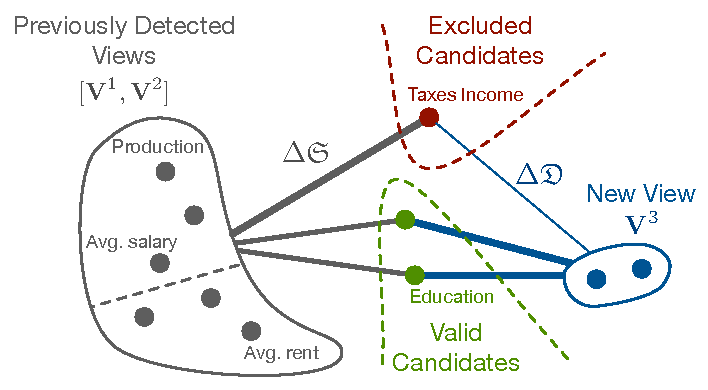
\includegraphics[width=\columnwidth]{Figures/Greedy}
  \caption{Illustration of Ziggy's greedy view composition algorithm, with
      $i=3$
  and $D=3$. Each point represents a column. The grey edges represent the
  amount of redundancy added by each candidate. The blue edges represent the
  amount of dissimilarity added by each candidate.}
  \label{pic:greedy}
\end{figure}
Ziggy operates in two steps. First, it computes the individual Zig-Components
for all the columns in the database. Then, it composes the views in a  greedy
manner. For each view, Ziggy detects which columns are eligible (i.e., do not
violate the redundancy constraint) and it adds those with the highest
Zig-Components.

The first step is straightforwards, but it is also by far the most time
consuming. We discuss in Section~\ref{sec:optimization} how to optimize it.
During the second step Ziggy creates the views by adding columns one by one.
Figure~\ref{pic:greedy} illustrates this approach. Suppose that Ziggy has
already obtained two views, $\rb{D}^1$ and $\rb{D}^2$, and it is currently
building a third one, $\rb{D}^3$. For each column in $\rb{D} \setminus \rb{D}^3
$, our algorithm computes two scores: the gain of dissimilarity $\Delta\mf{D}$
induced by adding the candidate to $\rb{D}^3$, and the gain of
redundancy~$\Delta\mf{S}$. Ziggy excludes the columns which exceed the
redundancy capacity, e.g., those for which $\mf{S}([\rb{D}^1, \rb{D}^2],
\rb{D}^3) + \Delta\mf{S} > L$, where $L$ is the dependency limit introduced in
Equation~\ref{prob2}. Ziggy then detects the best node among those that
remain (that is, that for which $\Delta\mf{D}$ is maximal) and adds it to the
view. It repeats the process until either the maximal number of columns is met, or
there are no more eligible columns.

In practice, care must be taken when computing $\Delta\mf{D}$, because one
column is often involved in several Zig-Components. Suppose for instance that we
are building a view $\rb{D}^{i}$, and we wish to compute $\Delta\mf{D}$ for
a given candidate $d$.  In our
implementation, if $d$ contains numeric values, then it will be associated with
at least two components: the difference between the means $\mf{z}_\mu$, and the
difference between the standard deviations $\mf{z}_\sigma$.  Additionally, we must
account for the difference between dependencies, for all the columns
already included in $\rb{D}^{i}$. Thus, if $z$ describes the normalized absolute
value of a Zig-Component $\mf{z}$, and if $\rb{D}^{i}_{num}$ and
$\rb{D}^{i}_{cat}$ respectively represent the numerical and categorical
variables of $\rb{D}^{i}$ the final score is:
%\begin{equation}
    \begin{multline}
\Delta\mf{D} = 
z_\mu(d_t, d_{\nott}) +
z_\sigma(d_t, d_{\nott}) \\
+ \sum_{d' \in \rb{D}^i_{num}} z_r([d_t, d_t'], [d_{\nott}, d_{\nott}'])
+ \sum_{d' \in \rb{D}^i_{cat}} z_V([d_t, d_t'], [d_{\nott}, d_{\nott}'])
\end{multline}
%\end{equation}
The last two terms of the equation depends on the current state of $ \rb{D}^i$.
Therefore we must update $\Delta\mf{D}$ after each step.

If we use the redundancy measure $\mf{S}_{hard}$, then we can avoid computing $
\Delta\mf{S}$ altogether: Ziggy can discard the redundant candidates before
it starts building the view.  Consider a candidate column $d$,
and let $\rb{D}^{1..i-1}$ describe the union of all previously encountered
views. If $\mf{S}_{hard} (\rb{D}^{1..i-1}, d) > L$, then the column is not
exploitable: adding it to the current view $\rb{D}^{i}$ will breach the
threshold, regardless of $\rb{D}^{i}$'s current state.  Conversely, if we have
$\mf{S}_{hard}(\rb{D}^{1..i-1}, d) < L$, then candidate is ``safe'', it will
never cause the dependency threshold to be breached.  Thus Ziggy, builds the
view in two separate steps: first it eliminates the redundant columns (i.e.,
those for which $\mf{S}_{hard} (\rb{D}^{1..i-1}, d) > L$), then it selects the
top $D$ candidates.  Unfortunately, this property does not hold for
$\mf{S}_{soft}$: we must recompute the value $\Delta\mf{S}$ for each column
after each update of~$\rb{D}^{i}$.

The choice of dependency measure also influences the correctness of our
algorithm. With $\mf{S}_{hard}$, Ziggy will return an optimal solution. This is
not the case with $\mf{S}_{hard}$.
{\color{red} I will write a little proof here. - Basically, we are dealing with
a variant of the knapsack problem.}

\subsection{Staging Computations}
\label{sec:optimization}

\begin{figure}[t!]
    \centering
    \begin{subfigure}[b]{0.8\columnwidth}
    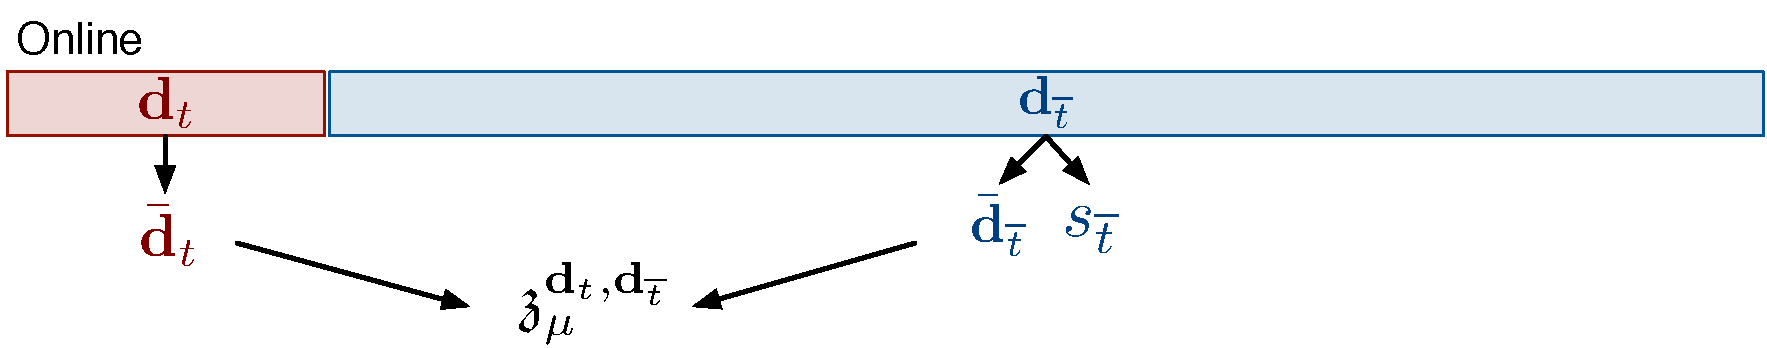
\includegraphics[width=\textwidth]{Figures/Staging}
    \caption{Computing $\mf{z}_\mu$ without staging.}
    \label{pic:withoutstag}
    \end{subfigure}

    \begin{subfigure}[b]{.8\columnwidth}
        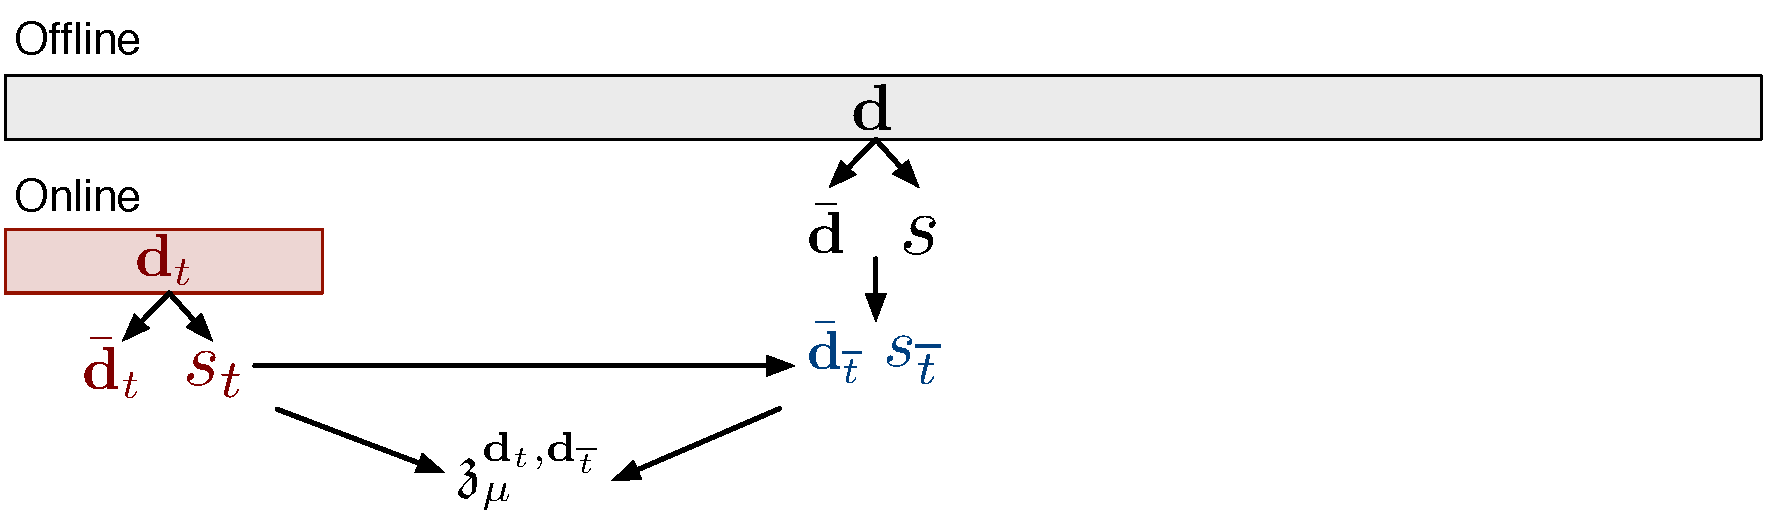
\includegraphics[width=\textwidth]{Figures/Staging2}
    \caption{Computing  $\mf{z}_\mu$  with staging.}
    \label{pic:withstag}
    \end{subfigure}
\end{figure}

We now discuss how to compute the Zig-Components for each column of the
database. This task is critical: in the best case, it requires a full scan of
the database. In the worse case it runs in $\mathcal{O}(N \cdot M^2)$:  to
obtain the scores $\mf{z}_r$ and $\mf{z}_V$, we need to compute and compare
every possible pair of correlations in $\rb{D}_t$ and $\rb{D}_{\nott}$.

Our idea is to prepare some computations offline, before the user starts
submitting queries.  Let us focus on the Zig-Component $\mf{z}_\mu$, which
reports the difference $\frac{\mu_{\nott} - \mu_{t}}{\sigma_t}$, for a given
column $d$ of the database.  Figure~\ref{pic:withoutstag} presents the naive
method to compute this component.  As soon as our user submits a selection, we
compute the average $\mu_t$ for those tuples, the values $\mu_{\nott}$ and
$\sigma_{\nott}$ for the rest of the database, and we apply the formula
$\frac{\mu_{\nott} - \mu_{t}}{\sigma_t}$  directly. Thus, we scan the whole
column.

Figure~\ref{pic:withstag} illustrates our staging strategy. Offline, we compute
the mean $\mu$ and the standard deviation $\sigma$ for the whole column~$d$.
Online, when the user submits a selection, we compute  $\mu_t$ and $\sigma_t$
only - thus, we read the selection and ignore the rest of the database. We then
reconstitute $\mu_{\nott}$ and $\sigma_{\nott}^2$, as follows:
\begin{gather}
    N_{\nott} = N - N_t\\
    \mu_{\nott}= \frac{ N \cdot \mu -  N_t \cdot \mu_t } { N - N_t } \\
    \sigma_{\nott}^2 = \sigma^2 - \sigma_t^2 -
    (\mu_t - \mu_{\nott})^2 \cdot \frac{N_t \cdot N_{\nott}}{N^2}
\end{gather}
We now have all the elements to compute the Zig-Component. To obtain these
equations, we used formulas designed to compute the mean and variance
incrementally~\cite{pebay2008formulas}, and we reversed them - in fact we
compute $\mu_{\nott}$ and $\sigma_{\nott}$ in a ``decremental'' fashion.

In effect, this method does not reduce the complexity of the algorithm, but it
greatly reduces the amount of tuples to read. The smaller the user's selection
is, the greater is the performance gain. Fortunately, we managed to extend it
for all the Zig-Components presented in Table~\ref{tab:dissim}.  We can derive
similar computations to update correlation
coefficients~\cite{pebay2008formulas}. To cope with categorical data, our
approach is slightly different. Offline, we compute a histogram for $d$. Online
we compute another histogram for $d_t$. From those, we can infer the
distribution of $d_{\nott}$'s values, and compute $\mf{z}_\chi$ and $\mf{z}_V$.


\section{Model Validation}
\label{sec:validation}
\begin{table*}[t!]
    \centering
    \begin{tabular}{c c c c p{9.5cm}}
      \hline
      Property & Type 1 & Type 2 & Test Statistic & Comment\\
      \hline
      Mean & Contin.  & - & $\frac{\mu_t - \mu_{\nott}}{\sigma}$ &
        Wald test~\cite{wasserman2013all}  \\
        Stand. Dev.& Contin.  & - & $\sigma_t / \sigma_{\nott}$ &
        F-test~\cite{wasserman2013all} \\
        Frequencies & Discrete & - & $\chi^2$ & Pearson's $\chi^2$
        test~\cite{wasserman2013all}\\
      \hline
      Dependence  & Contin. & Contin & $\frac{Z - Z'}{\sigma_{Z - Z'}}$ & $Z_1$
      and $Z_2$ are the Fisher Z-transformations of the correlations $r$ and
      $r'$~\cite{fisher1915frequency}  \\
      Dependence  & Contin. & Both &  $\frac{V-V'}{\sigma_{V-V'}}$ & $V$ is
      Cram\'er's V. To test it, we exploit Fisher's
      Normal approximation of $\sqrt{\chi^2}$~\cite{patel1996handbook}.\\ 
      \hline
    \end{tabular}
\caption{Our choice of tests, corresponding to each Zig-Component.}
    \label{tab:tests}
\end{table*}

We now focus on the following problem: for a given view $\rb{D^i}$, how
\emph{significant} is the Zig-Dissimilarity $D = \mf{D}( \rb{D}^i_t  ;
\rb{D}^i_{\overline{t}})$? A high value may indicate that $\rb{D}^i_t$ and
$\rb{D}^i_{\overline{t}}$ come from two different distributions.  But it could
also be caused by chance. How confident are we of this result? Answering this
question has two practical uses. First, a confidence score would let us decide
when to stop generating views. Second, it could help users
interpret Ziggy's results.

In fact, the statistics literature proposes a completely ge\-ne\-ric way to solve
this problem: permutation testing. This methods works with the Zig-Dependency,
but it also handles other divergence measures. The main idea is to
repeatedly shuffle the rows of $D^i$, without modifying $\rb{t}$. Thus, the
tuples are randomly affected to $\rb{D}^i_t$ and $\rb{D}^i_{\overline{t}}$. We
then observe how the dissimilarity varies: if the random permutations have no
effect on $D$, then there is high chance that the dissimilarity was caused by
chance.  Oppositely, if $D$ is very sensitive to the affectation of the tuples,
then we have a high confidence in our result. We refer the interested
reader to Wasserman~\cite{wasserman2013all} for more details.

Permutation testing offers plenty of advantages, but shuffling the rows is
computationally heavy. In our implementation, we used an alternative approach. The
main idea is to use the composite nature of the Zig-Dissimilarity, and test
each Zig-Component individually. We then aggregate these scores in a synthetic
confidence indicator. Therefore we do not test the Zig-Dissimilarity directly -
instead we focus on its underlying effects.  This method is much lighter because we can use
known asymptotic results, or at least approximations thereof. For instance, we
know that under certain assumptions, the difference between the means is
approximately normally distributed. Therefore we can use Wald
test~\cite{wasserman2013all}, which only requires an extra $\mathcal{O}(1)$
computation.  Similarly, we can use a F-test for the ratio of the variances,
or a $\chi^2$ test for the differences in categorical distributions.
Table~\ref{tab:tests} summarizes our choices. 

To aggregate the tests, we report the minimum observed p-value. We must note
that this approach is very conservative. More flexible alternatives include
the Bonferroni corrections, or the Benjamini-Hochberg
method~\cite{wasserman2013all}.

\section{Setting Parameters}
\label{sec:parameters}

Ziggy's model relies on three parameters: the total number of views $K$ to
generate, the width of the views $D$, and the dependency threshold $L$. We know
discuss how to set these parameters.

\textbf{Number of Views K.} Interpreting this parameter is straightforward: a
high $K$ leads to more information, but also potentially insignificant views
and a lengthier output. When should we stop? We propose to generate as many
views as possible, and delegate the final decision to the users - after all, we
have little idea about what they seeking. In practice, we can do so lazily:
we start with a small selection of views (e.g., as many as the display can
contain), and we generate the remainder on demand, for instance with a ``show
me more'' button.  In our experience, the number of views stays
manageable because the algorithm is blocked by the redundancy constraint:
after a certain number of views, Ziggy finds no more columns to exploit. If the
views have a low confidence (as detailed in Section~\ref{sec:validation}), then
Ziggy issues a warning.

\textbf{Size of the Views D.}  A low D with leads to many small views, while a
large value leads to a few large views. Which value describes the data most
accurately? In our implementation, we set this parameter in an adaptive
fashion, using a method presented by Zhu and Ghodsi~\cite{zhu2006automatic}.
The main idea is the following. When building a view, we keep track of the
gains $\Delta\mf{D}_d$ induced by each column $d$.  We then detect change
points in the sequence (e.g., ``jumps'' or ``elbows'').  If we observe such a
behavior, we truncate the current view and start a new one.  The advantage of
this method is that the value of $D$ can adapt to each subspace. However, it is
only a heuristic. Fortunately, inaccuracies have little consequence in
practice: if the dependency constraint is weak, then the excluded columns are
simply pushed to the next view.

\textbf{Dependency threshold L.} Admittedly, there is no optimal way to set
this parameter: it depends entirely on the user and the exploration context. By
default, we use $\mf{S}_{hard}$, and we limit to $L=0.99$. This setting
enforces that the views are non-overlapping, but it adds no other constraint -
we see this as a safe option.


\section{Report Generation}
\label{sec:reporting}
We now detail how Ziggy describes the views.
{\color{red} I have 1-2 pages of content for this Section. Work in progress.}

\section{Use Case}
\label{sec:usecase}

\begin{table}[!ht]
    \centering
    \small
    \begin{tabular}{p{4cm} c c c} 
        \hline
        \multirow{3}{*}{Columns}  & Except. & Weak  & \multirow{3}{*}{Score}\\
                                  & Comp.   & Comp.& \\
                                  & (\%)    & (\%)& \\
        \hline
        Patent\_applications\_per\_million & \multirow{3}{*}{83.3}
        &\multirow{3}{*}{0} & \multirow{3}{*}{25.4} \\
        PCT\_patent\_applications&&&\\
        Personal\_earnings &&&\\
        \hline
        Dwellings\_no\_basic\_facilities&
        \multirow{4}{*}{64.2} &\multirow{4}{*}{7.1} & \multirow{4}{*}{18.9} \\
        Educational\_attainment&&&\\
        Emp.\_work\_very\_long\_hours&&&\\
        Life\_expectancy&&&\\
        \hline
        Average\_hours\_worked&
        \multirow{4}{*}{50} &\multirow{4}{*}{42.2} & \multirow{4}{*}{12.4} \\
        Population\_growth\_rates&&&\\ 
        Working\_age\_population&&&\\
        Pop\_under\_the\_age\_of\_15&&&\\
        \hline
        Assault\_rate, Homicide\_rate &
        \multirow{2}{*}{77.7} &\multirow{2}{*}{11.1} & \multirow{2}{*}{12.1} \\
        Current\_\-account\_balance&&&\\
        \hline
        Export\_Pharmaceutical&
        \multirow{4}{*}{57.1} &\multirow{4}{*}{57.1} & \multirow{4}{*}{11.4} \\
        Incidence\_part\_time\_emp&&&\\ 
        Long\_term\_unemp&&&\\ 
        Production\_crude\_oil&&&\\ 
        \hline
        Air\_pollution, Job\_security&
        \multirow{2}{*}{77.7} &\multirow{2}{*}{11.1} & \multirow{2}{*}{10.1} \\
        Student\_skills&&&\\
        \hline
        Employment\_rate&
        \multirow{3}{*}{66.6} &\multirow{3}{*}{33.3} & \multirow{3}{*}{7.1} \\
        Total\_primary\_energy\_supply&&&\\ 
        Trade\_Balance.\_Pharmaceutical&&&\\ 
        \hline
        Triadic\_patent\_year&
        \multirow{2}{*}{28.5} &\multirow{2}{*}{75.5} & \multirow{2}{*}{6.2} \\
        Time\_devoted\_to\_leisure&&&\\ 
        \hline
        Renewable\_energy\_supply&
        \multirow{3}{*}{33.3} &\multirow{3}{*}{55.5} & \multirow{3}{*}{5.5} \\
        Voter\_turnout&&&\\ 
        Total\_tax\_revenue&&&\\ 
        \hline
        Consultation\_on\_rule\_making&
        \multirow{3}{*}{7.1} &\multirow{3}{*}{78.5} & \multirow{3}{*}{5.3} \\
        Implicit\_GDP\_Price\_Indices&&&\\
        Years\_in\_education&&&\\
        \hline
        Quality\_of\_support\_network&
        \multirow{2}{*}{33.3} &\multirow{2}{*}{55.5} & \multirow{2}{*}{4.5} \\
        Taxes\_on\_income\_and\_profits&&&\\
        \hline
        Value\_Added\_of\_Industry&
        \multirow{3}{*}{0} &\multirow{3}{*}{100} & \multirow{3}{*}{2.9} \\
        Exchange\_Rates&&&\\
        Gross\_Domestic\_Product&&&\\
        \hline
    \end{tabular}
    \caption{Detail of Ziggy's views, sorted by decreasing order of score. The
    two middle columns indicate the proportion of Zig-Components considered as
Exceptional and Weak.}
    \label{tab:ziggysviews}
\end{table}
\begin{figure*}[!ht]
  \centering
  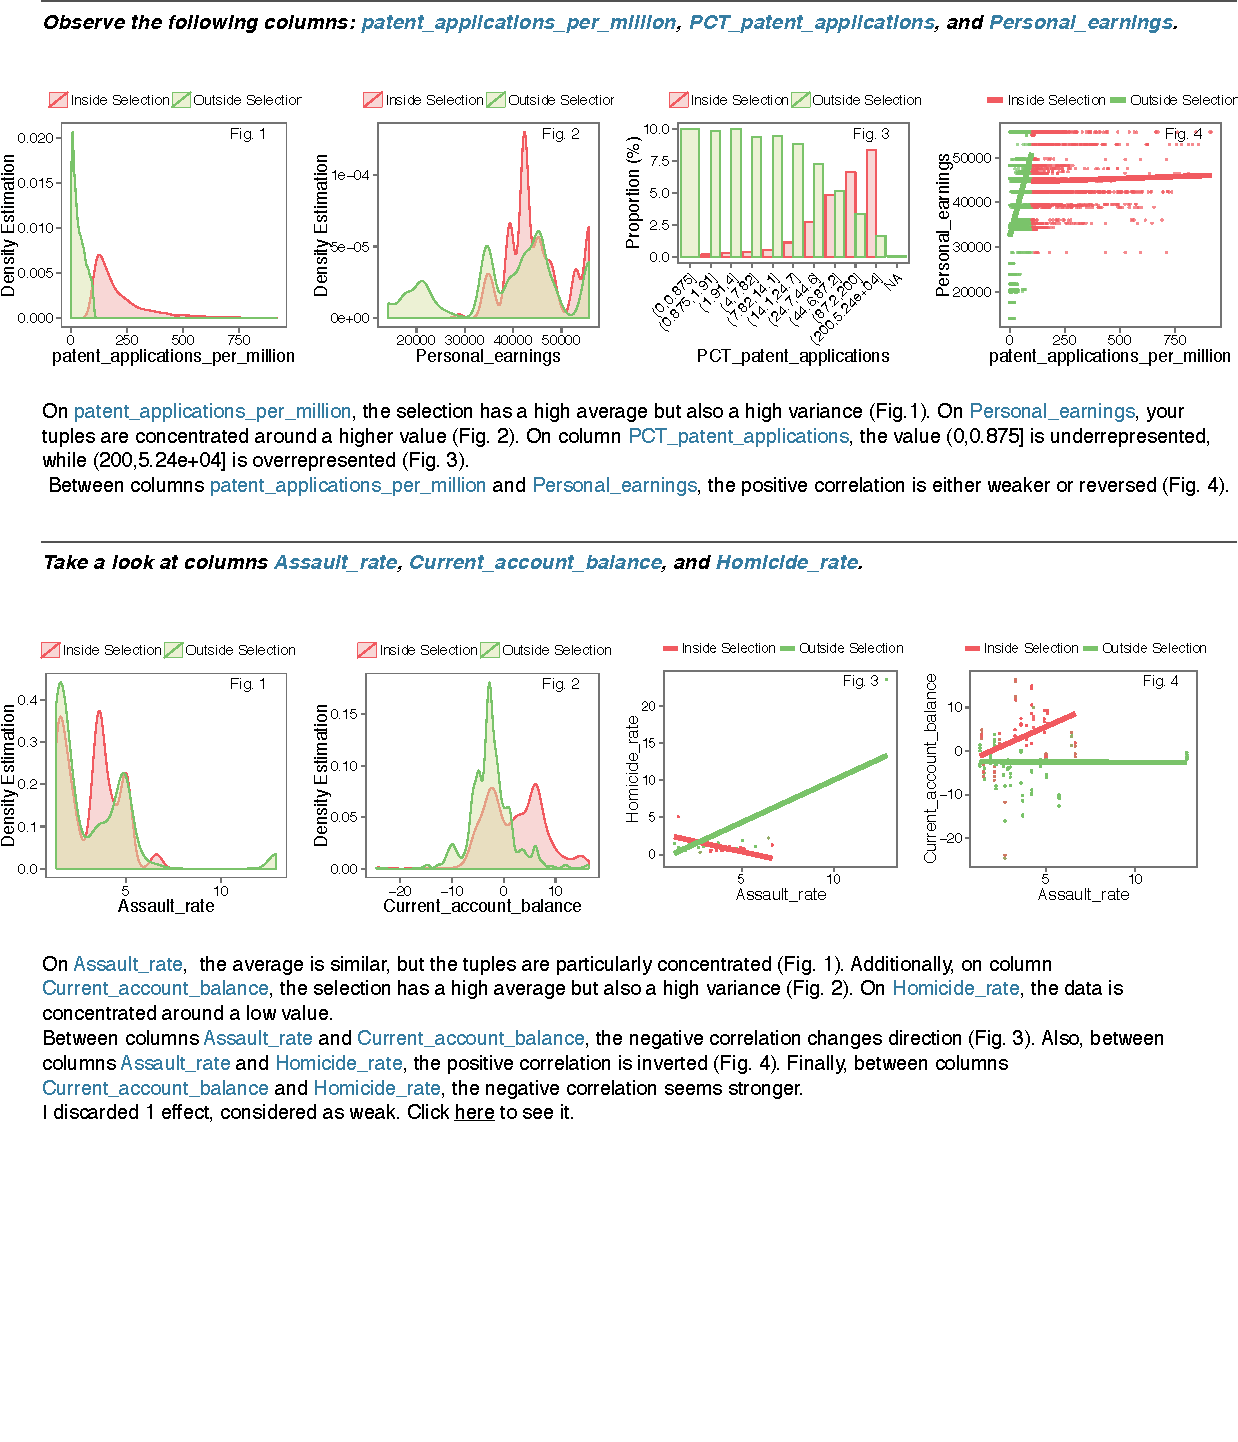
\includegraphics[width=1.8\columnwidth]{Figures/ZigUseCase}
  \caption{Ziggy's explanations for Views 1 and 4}
  \label{pic:zigdetail}
\end{figure*}
We now present a real-life use case. Our general aim is to understand what
demographic, social and economic factors lead to innovation. More specifically,
we are interested in patents: in which parts of the world do individuals
submit patents? What lessons can we learn?

To answer these questions, we aggregated several databases from the OECD, an
international economic organization. All the data we used can be found
online\footnote{http://stats.oecd.org/}. Our core dataset is the
\texttt{Patents per Region} table, which contains 15 years of patent statistics
for 2,180 regions in 31 countries. We augmented this table with several other
region-level databases: \texttt{Demographics per Region} and \texttt{Labour per
Region}. Finally, we added country-level information: we used the sets
\texttt{Better Life}, \texttt{Well Being} and \texttt{Innovation Indicators}.
We obtain a table with about 6,823 rows and 519 columns, including mixed types
and missing values. We filtered out the categorical columns with
more than 20 distinct values (e.g., primary keys, countries and region names).
Our selection of tuples contains the top 10\% regions for the statistic
\texttt{patent applications per million inhabitant}. We set $D=6$ with the
adaptive stopping method described in Section~\ref{sec:parameters}, and we used
$\mf{S}_{hard}$, with a maximum value of $L=0.75$.

Ziggy detects a total of 12 views, which columns are reported in
Table~\ref{tab:ziggysviews}. Some of Ziggy's choice are not surprising. For
instance, the first column mentioned in the Table is precisely the variable we
used to define our selection. The second one,
$\texttt{PCT\_patent\_applications}$ is highly similar (the PCT is an
international patent treaty, which allows transnational patents). Likewise, we
expected some relationship between education and innovation (views 2, 6 and
10). However, some effects are less straightforward. How does
\texttt{Emp.\_work\_very\_long\_hours} impact innovation? Are patents produced
at work, or during hobby time? Similarly, how do our innovative regions behave
on the variable~\texttt{Job\_security}?

Figure~\ref{pic:zigdetail} presents Ziggy's explanations for two views. To
obtain this figure, we made only two edits: we removed some plots to save
space, and we inserted references to the charts in the text. Consequently, the
figure illustrates accurately what Ziggy's users would obtain. The first view
reflects the fact that innovative regions also have a high income. Ziggy
expresses this through its comments about the
variable~\texttt{Personal\_earnings}, but also through the last chart. As it
points out, there is a correlation between patent applications and income, but
this correlation disappears when we focus on innovative regions. Then, the
regression line is flat, with a high offset, which indicates that all these
regions are relatively rich, regardless of their patent statistics.

The second view offers a different perspective. The first and third charts show
that innovative regions tend to be safer. Indeed, the variable
\texttt{Assault\_rate} is usually correlated with \texttt{Homicide\_rate}. But
in our case, this correlation is inverted. This reflects the fact that assaults
do exist in our innovative regions, but little of them actually lead to a
homicide. The last chart is more puzzling: there normally exists no
relationship between \texttt{Assault\_rate} and
\texttt{Current\_account\_balance}. And indeed, we expect these variables to be
independent, because they describe completely different topics. And yet, in the
innovative regions, a clear correlation appears. How can we interpret this
effect? If this dependence completely spurious? Alternatively, are those
variables cofounded by a third, hidden variable? Or maybe sane public accounts
causes anger among inventors? As absurd as this last hypothesis may seem, we
have no way to discard it. We leave this question open for future investigations.

\section{Experiments}
\label{sec:experiments}
{\color{red} I easily have 2-3 pages of content for this section. Work in
progress.}

\section{Related Work}
\label{sec:related-works}
{\color{red} Big TODO: contrast with Bailey's approach.
I still have to read about metric learning.}


\section{Conclusion}
\label{sec:conclusions}




%\section*{[Private] Appendix: Ziggy vs.Claude}
%\label{zigvsclaude}
%We may now wonder: if we set $\mf{D}$ as the KL divergence, what is the
%difference between Claude and Ziggy?  Suppose that we ignore the penalty factor
%(we set $\lambda=0$). Then Ziggy tries to maximize:
%$$
%KL\big(\rb{x} | t=0 \ ; \  \rb{x} | t=1 \big)
%$$
%Intuitively, this is the distance between $\rb{x} | t=0$ and $\rb{x} | t=1$.
%On the other hand, Claude maximizes $I(\rb{x}, t)$. With a bit of playing
%around, we can show that this is equivalent to maximizing:
%$$
%    KL\big(\rb{x} | t=0 \ ; \  \rb{x} \big) + 
%        KL\big(\rb{x} | t=1 \ ; \  \rb{x} \big)
%$$
%Here, we are interested in the distance between $\rb{x} | t=i$ and a central
%distribution $\rb{x}$. 
%
%There is a triangular relationship between these expressions:
%\begin{figure}[h!]
%  \centering
%  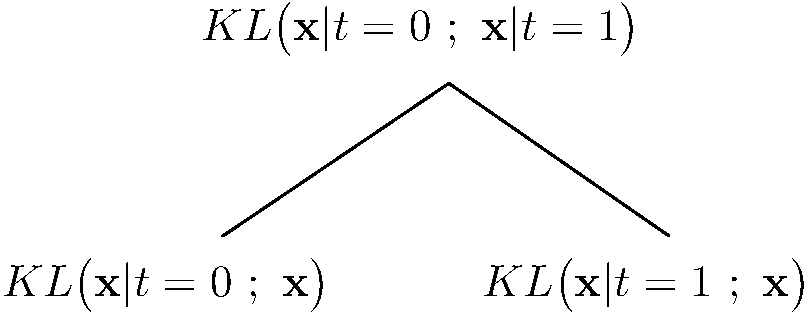
\includegraphics[width=0.6\columnwidth]{Figures/Triangle}
%  \label{pic:triangle}
%\end{figure}
%
%I wonder if they are not actually equivalent!




\section{Acknowledgements}
This publication was supported by the Dutch national program COMMIT.

\bibliographystyle{abbrv}
\balance
\bibliography{MME}
\end{document}
